% !TeX root = Protokoll.tex

\begin{figure}[h!]
	\centering
	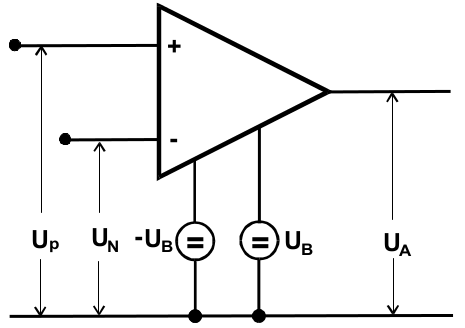
\includegraphics[width= 0.5\textwidth]{../Grafiken/OP_Schaltung.png}
	\caption{Hier ist die skizzierte Schaltung eines Operationsverstärkers dargestellt. \cite{V51}\label{fig:OP_Schaltung}}
\end{figure}
\noindent
In \cref{fig:OP_Schaltung} ist die Schaltung für einen Operationsverstärker dargestellt.
Ein Operationsverstärker wird durch zwei konstante Betriebsspannungen $U_\text{B}$ und $-U_\text{B}$ betrieben.
Weiter ist die resultierende Ausgangsspannung $U_\text{A}$ als
\begin{align}
	U_\text{A}=V(U_\text{p}-U_\text{N})
	\label{eq:leerlauf_verstaerkung_opv}
\end{align}
gegeben. 
Dabei ist $U_\text{p}$ die Spannung des nicht-invertierenden Eingangs, $U_\text{N}$ die Spannung des invertierenden Eingangs und $V$ ist die Leerlaufverstärkung.
Dabei wird die Spannung verstärkt, wenn 
\begin{align*}
	-U_\text{B}<U_\text{A}<U_\text{B},
\end{align*}
außerhalb dieses Intervalls ist die Ausgangsspannung $U_\text{A}=\pm U_\text{B}$.
Die Kennlinie ist in \cref{fig:Kennlinie} dargestellt.
\begin{figure}
	\centering
	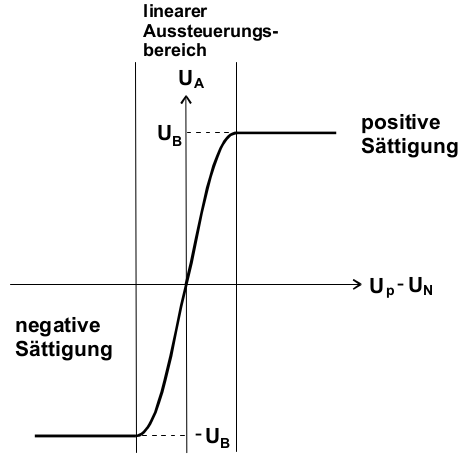
\includegraphics[width = 0.5\textwidth]{../Grafiken/Op_Kennlinie.png}
	\caption{Hier ist die Kennlinie eines Operationsverstärkers dargestellt. \cite{V51}\label{fig:Kennlinie}}
\end{figure} 
Ein  Operationsverstärker wird, neben der Leerlaufverstärkung $V$, durch mehrere Kenngrößen beschrieben.
Den beiden Eingangswiederständen $r_{\text{e}_{{}_\text{p}}}$ und $r_{\text{e}_{{}_\text{N}}}$ sowie den Ausgangswiederstand $r_\text{a}$.
Die Leerlaufverstärkung $V$ ist im allgemeinen Fall sehr groß und abhängig von der Frequenz, weswegen sie für einen idealen Operationsverstärker als unendlich angenommen wird.
Die Eingangswiderstände sind sehr groß, weswegen die idealen als unendlich angenommen werden.
Der Ausgangswiederstand hingegen ist klein, weshalb der ideale als null angenommen werden kann.
\begin{align}
	V_\text{id}=\infty,~ r_{\text{e}_\text{id}}=\infty,~ r_{\text{a}_\text{id}}=0
\end{align}
Für einen realen Operationsverstärker müssen weitere Kenngrößen eingeführt werden.
Aufgrund von Asymmetrien in einem realen Operationsverstärker ist die Ausgangsspannung ungleich null, auch wenn zwei gleiche Spannungen $U_\text{Gl}$ an den Eingängen angelegt werden.
Deshalb ist es hilfreich die Gleichtaktverstärkung $V_\text{Gl}$ zu definieren 
\begin{align}
	V_\text{Gl}:=\frac{\Delta U_\text{A}}{\Delta U_\text{Gl}}.
\end{align}
Weiter treten aufgrund der endlichen Eingangswiederstände $r_e$ in einem realen Operationsverstärker Eingangsströme $I_\text{N}$ und $I_\text{P}$ auf.
Daraus lässt sich der Eingangsruhestrom $I_\text{B}$ definieren als
\begin{align}
	I_\text{B}:=\frac{1}{2}\left( I_\text{p} + I_\text{N} \right)
\end{align}
und ebenfalls lässt sich der Offsetstrom $I_0$ definieren
\begin{align}
	I_0:=I_\text{p}-I_\text{N},~ \text{ für }U_\text{N}=U_\text{p}=0.
\end{align}
Durch die Ströme $I_\text{p}$ und $I_\text{N}$ lässt sich der Differenzeneingangswiderstand $r_\text{D}$ definieren als
\begin{align}
	r_\text{D}:=
	\begin{cases}
		\frac{\Delta U_\text{p}}{\Delta I_\text{p}}\text{, wenn } U_\text{N}=0\\
		\\
		\frac{\Delta U_\text{N}}{\Delta I_\text{N}}\text{, wenn } U_\text{p}=0
	\end{cases}
\end{align}
genauso wie der Gleichtaktwiderstand $r_\text{Gl}$
\begin{align}
	r_\text{Gl}=\frac{\Delta U_\text{Gl}}{I_\text{Gl}}.
\end{align}
Wobei gilt, das $U_\text{Gl}=U_\text{p}=U_\text{N}$ und $I_\text{Gl}=I_\text{p}+I_\text{N}$ ist.
Weil für einen realen Operationsverstärker die Ausgangsspannung $U_\text{A}$ nicht null ist, wenn $U_\text{N}=U_\text{p}$ ist, wird die Offsetspannung $U_0$ eingeführt:
\begin{align}
	U_0:=U_\text{p}-U_\text{N}\text{, sodass }U_\text{A}=0.
\end{align}
\subsection{Linearverstärker}
\begin{figure}[h!]
	\centering
	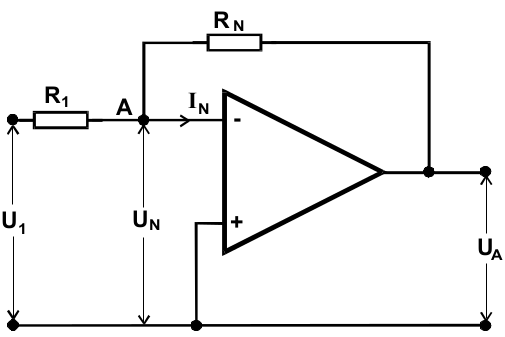
\includegraphics[width = 0.6\textwidth]{../Grafiken/Gegengekoppelter_Invertierter_Liniearverstaerker.png}
	\caption{Hier ist die Schaltung eines gegengekoppelten, invertierter Linearverstärker skizziert. \cite{V51}\label{fig:gegen_gekoppelter_invertierter_Linarverstärker}}
\end{figure}
\noindent
Aufgrund der großen Leerlaufverstärkung, kann ein Operationsverstärker nicht direkt als Linearverstärker eingesetzt werden.
Dies wird umgangen, indem die Schaltung nach \cref{fig:gegen_gekoppelter_invertierter_Linarverstärker} verwendet wird.
Dabei wird ein Teil der Ausgangsspannung mithilfe eines Gegengenkopplungszweig auf den invertierenden Eingang zurückgegeben.
Deswegen wird die Schaltung auch gegengekoppelter, invertierter Linearverstärker genannt.
Das sorgt dafür das bei größerer Ausgangsspannung die Eingangsspannung abnimmt.
Aufgrund der großen Leerlaufverstärkung $V$ ist die Eingangsspannung des invertierten Eingangs $U_\text{N}$ nah zu 
null, da sich aus \cref{eq:leerlauf_verstaerkung_opv} mit $U_{\mathrm{P}}$ (aus der Schaltung in \cref{fig:gegen_gekoppelter_invertierter_Linarverstärker}) 
\begin{empheq}{equation}
	U_\text{N} = - \frac{U_{\mathrm{A}}}{V}
\end{empheq}
ergibt.
Genau so ist auch der Eingangsstrom $I_\text{N}\approx0$, da der Eingangswiderstand ebenfalls sehr groß ist.
Mithilfe der Kirchhoffschen Knotenregel, angewandt auf Punkt A aus \cref{fig:gegen_gekoppelter_invertierter_Linarverstärker} kann gezeigt werden, dass für die Verstärkung $V'$ gilt
\begin{align}
	V' = -\frac{R_\text{N}}{R_1}.
	\label{eq:gegengekoppelt_verstaerkung}
\end{align}
Dies gilt für einen idealen Operationsverstärker.
Für einen realen mit endlichen Widerständen und weiterhin verschwindendem Strom $I_\text{N}$ am invertierenden Eingang gilt 
\begin{align}
	\frac{1}{V'}\approx\frac{1}{V}+\frac{R_1}{R_\text{N}}.
	\label{eq:leerlauf_verstaerkung}
\end{align}
Es lässt sich erkennen, dass die Verstärkung $V'$ für den idealen und realen Operationsverstärker gleich sind wenn gilt $R_\text{N}/R_1\ll V$.
Da die Eigenschaften der Schaltung hauptsächlich durch die äußere Beschaltung festgelegt werden,
macht die Gegenkopplung Verstärkung unabhängig von äußeren Einflüsse auf den Operationsverstärker,
dies bedeutet, dass die Schaltung auf diese Art stabilisiert wird.
Der Ausgangswiederstand wird aufgrund der Gegenkopplung durch den Faktor $g$ verkleinert.
Dabei ist $g$ definiert als
\begin{align}
	g:= \frac{V}{V'}.
\end{align}
Ein weiterer Vorteil der Gegenkopplung ist, dass die Schwankung der Leerlaufverstärkung durch den Faktor $g$ vermindert wird.
\begin{align}
	\frac{\Delta V'}{V'}=\frac{1}{g}\frac{\Delta V}{V}
\end{align}

Zum Schluss wird das Frequenzband durch den Faktor $g$ vergrößert.
Dies ist in \cref{fig:Frequenzgang} dargestellt. Die Frequenz bis zu der das Signal unverzerrt verstärkt 
wird (maximale Frequenz des Frequenz im Frequenzband), wird als Grenzfrequenz $f_{\mathrm{g}}$ bezeichnet. 
Für die Grenzfrequenz $f_{\mathrm{g}} = \sfrac{V'}{\sqrt{2}}$, gilt dass das Produkt aus $f_{\mathrm{g}}$ und der Verstärkung $V'$ eine Konstante ist, die gleich der Transitfrequenz ist.
Bei dieser ist die Verstärkung $V'$ auf den Wert 1 abgesunken.
\begin{figure}[h!]
	\centering
	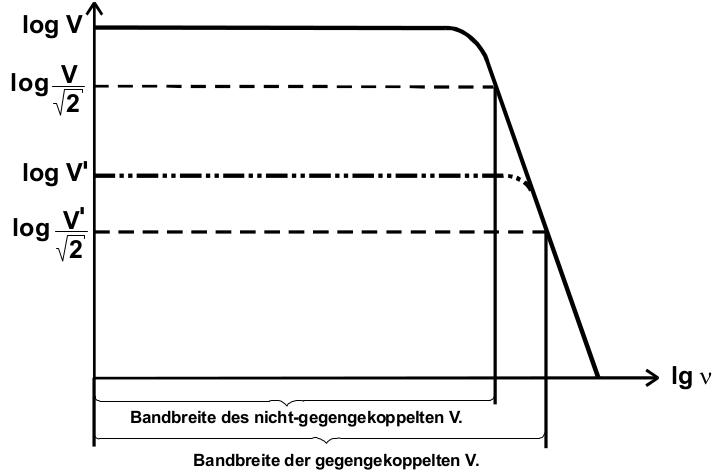
\includegraphics[width = 0.6\textwidth]{../Grafiken/Frequenz_Liniearverstaerker.png}
	\caption{Frequenzband des Linearverstärkers. \cite{V51}\label{fig:Frequenzgang}}
\end{figure}\\
\indent
Ein Nachteil des gegengekoppelten, invertierten Linearverstärkers ist der geringe Eingangswiederstand.
Dies verfälscht die Spannungsmessung an einer hochohmigen Spannungsquelle.
\begin{figure}[h!]
	\centering
	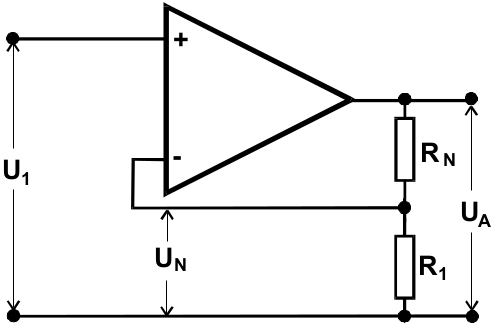
\includegraphics[width = 0.6\textwidth]{../Grafiken/nicht_invertierter_Linearverstaerker.png}
	\caption{Hier ist die Schaltung eines nicht-invertierender Elektrometerverstärkers dargestellt. \cite{V51}\label{fig:Elektrometerverstärker}}
\end{figure}
Deshalb wird für eine solche Messung eine Schaltung nach \cref{fig:Elektrometerverstärker} verwendet.
Dieser Aufbau wird Elektrometerverstärker genannt.
Bei dieser Schaltung ist der Eingangswiederstand gegeben durch
\begin{align}
	r_\text{e}\approx 2r_\text{Gl}\propto \SI{10}{\giga\ohm}.
\end{align}
Die Verstärkung $V'$ unter der Voraussetzung eines idealen Operationsverstärkers ist gegeben durch
\begin{align}
	V'=\frac{R_\text{N}+R_1}{R_1 }.
\end{align}
\indent
Wenn kleine Ströme gemessen werden sollen, muss der Eingangswiderstand klein sein.
Um dies zu erreichen wird eine Schaltung nach \cref{fig:Amperemeter} verwendet.
\begin{figure}[h!]
	\centering
	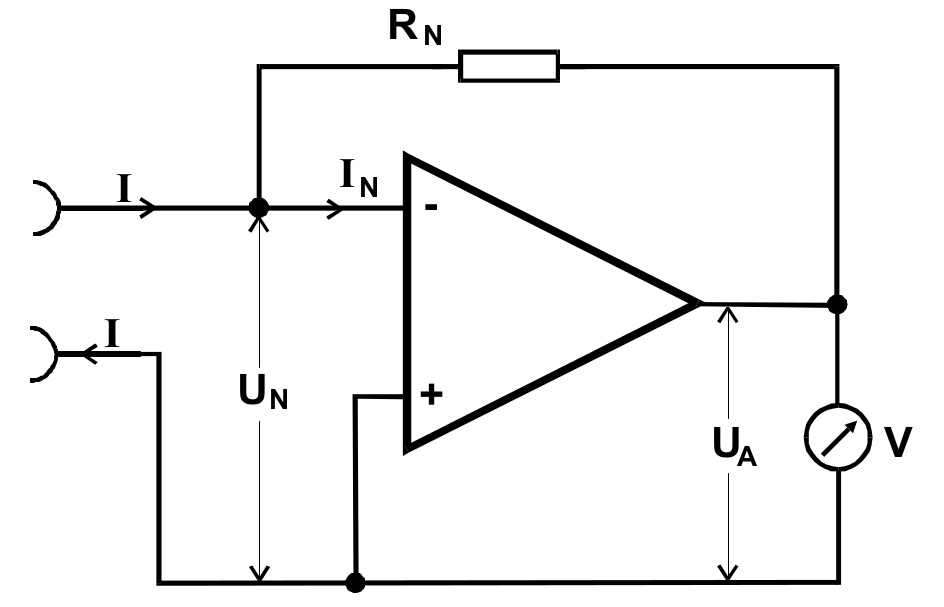
\includegraphics[width = 0.6\textwidth]{../Grafiken/Amperemeter.png}
	\caption{Hier ist die Schaltung eines Amperemeters dargestellt. \cite{V51}\label{fig:Amperemeter}}
\end{figure}
\FloatBarrier
Die Ausgangsspannung $U_\text{A}$ ist dann
\begin{align}
	U_\text{A}=IR_\text{N}.\label{eq:amperemeter_strom}
\end{align}
Dass bedeutet, die Ausgangsspannung $U_\text{A}$ ist proportional zum Eingangsstrom $I$.
Für den Eingangswiederstand gilt\\
\begin{align*}
	r_\text{e}=\frac{R_\text{N}}{V}.
	\label{eq:eingangswiderstand}
\end{align*}
\subsection{Umkehr-Integrator und Umkehr-Differenzierer}
\label{sec:Umkehr-Integrator}
\begin{figure}[h!]
	\centering
	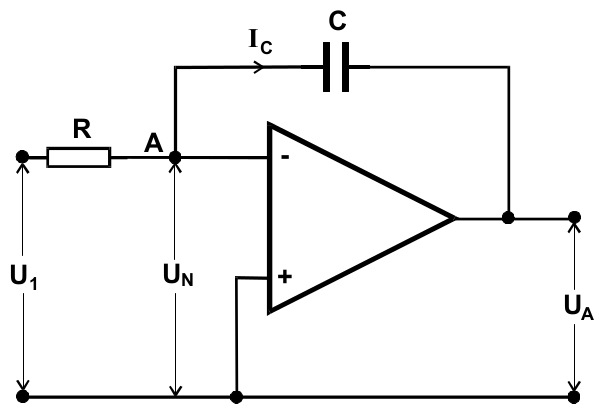
\includegraphics[width=0.5\textwidth]{../Grafiken/Umkehr_Integrator.png}
	\caption{Hier ist die Schaltung des Umkehr-Integrators dargestellt. \cite{V51} \label{fig:Umkehr_Integrator}}
\end{figure}
\noindent
Mithilfe eines Operationsverstärkers kann auch ein Signal integriert werden.
Dazu wird ein Rückkopplungszweig mit Kondensator mit der Kapazität $C$ geschaltet, wie in \cref{fig:Umkehr_Integrator} dargestellt.
Daraus folgt für die Ausgangsspannung
\begin{align}
	U_\text{A}=-\frac{1}{RC}\int U_1(t)dt.
\end{align}
Aufgrund des Minuszeichen wird die Schaltung Umkehr-Integrator genannt.
Wenn eine Sinusspannung $U_1=U_0\sin(\omega t)$ angelegt wird, folgt für die Ausgangsspannung
\begin{align}
	U_\text{A}=\frac{U_0}{\omega RC}\cos(\omega t).
\end{align}
Es lässt sich erkennen, dass die Amplitude vom Inversen der Frequenz $\omega$ abhängig ist.\\\indent
Durch vertauschen des Kondensators und des Widerstands lässt sich ein Umkehr-Differenzierer bauen, wie in \cref{fig:Umkehr_Diff} dargestellt.
\begin{figure}[h!]
	\centering
	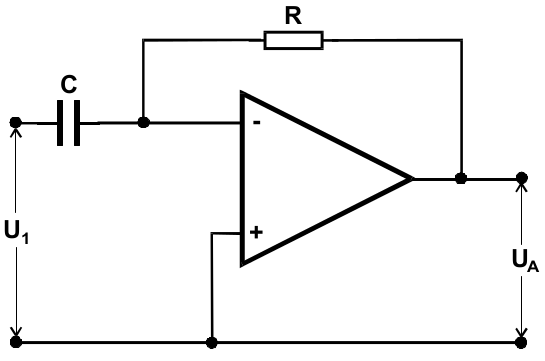
\includegraphics[width = 0.6\textwidth]{../Grafiken/Umkehr_Differentierer.png}
	\caption{Hier ist die Schaltung eines Umkehr-Differenzierers skizziert. \cite{V51}\label{fig:Umkehr_Diff}}
\end{figure}
Die Ausgangsspannung ist gegeben durch
\begin{align}
	U_\text{A}=-RC\frac{dU_1}{dt}.
\end{align}
Es lässt sich anhand des Beispiels der Sinusspannung erkennen, dass das Ausgangssignal linear zur Frequenz $\omega$ ist.
\subsection{Schmitt-Trigger}
\label{sec:Schmitt}
\begin{figure}[h!]
	\centering
	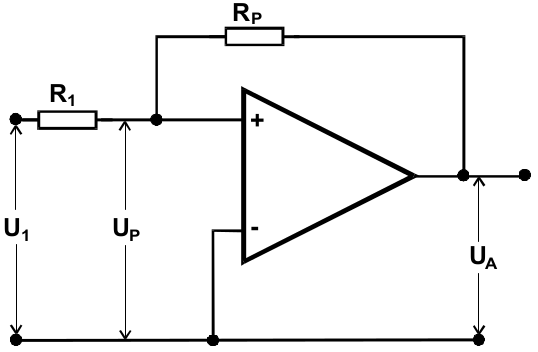
\includegraphics[width = 0.6\textwidth]{../Grafiken/Schmitt-Trigger.png}
	\caption{Hier ist die Schaltung für einen Schmitt-Trigger dargestellt. \cite{V51}\label{fig:Schmitt-Trigger}}
\end{figure}
\noindent
Ein Schmitt-Trigger vergrößert die Verstärkung $V'$ so, dass die Ausgangsspannung entweder $U_\text{B}$ oder $-U_\text{B}$ sein kann.
Dies wird erreicht in dem eine Rückkopplung in den nicht-invertierten Eingang des Operationsverstärker stattfindet, wie in \cref{fig:Schmitt-Trigger} dargestellt.
Die Ausgangsspannung geht in die Sättigung nach:
\begin{align}
	U_\text{A}=
	\begin{cases}
		+U_\text{B}\text{, wenn } U_1 > +\frac{R_1}{R_\text{P}}U_\text{B} \\
		-U_\text{B}\text{, wenn } U_1 < -\frac{R_1}{R_\text{P}}U_\text{B}
	\end{cases}\label{eq:kippspannug}
\end{align}
Für die Beträge der Eingangsspannung $\abs{U_1} < \frac{R_1}{R_\text{P}}U_\text{B}$ hält der Schmitt-Trigger
die Ausgangsspannung $U_\text{A}$ konstant auf dem entsprechenden Wert. 

\subsection{Operationsgenerator als Dreiecksgenerator}
\begin{figure}[h!]
	\centering
	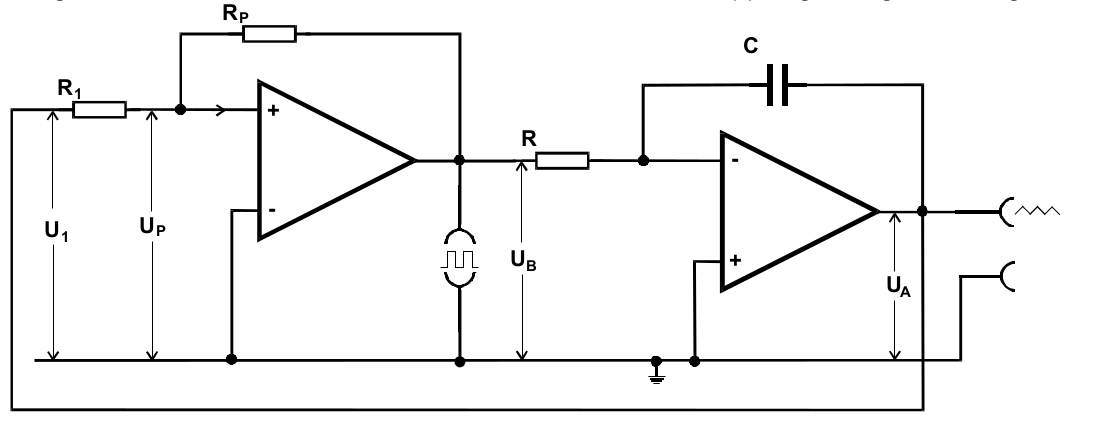
\includegraphics[width = 0.6\textwidth]{../Grafiken/Dreieckgenerator.png}
	\caption{Hier ist die Schaltung eines Dreiecksgenerator dargestellt. \cite{V51} \label{fig:Dreieck}}
\end{figure}
\noindent
Mithilfe mehrerer Operationsverstärker, kann ein Dreieckgenerator gebaut werden.
Die Schaltung besteht im wesentlichen aus einem Schmitt-Trigger und einem Umkehr-Integrator und ist in \cref{fig:Dreieck} dargestellt.
(Dabei werden die beiden Ausgangsspannungen auf den nicht-invertierten Eingang des ersten Operationsverstärkers geleitet.)
Der Schmitt-Trigger liefert eine konstante Spannung, die vom Umkehr-Integrator integriert wird.
Das bedeutet nach dem Umkehr-Integrator steigt beziehungsweise fällt die Spannung linear. 
Diese Spannung wird als Eingangsspannung auf den Schmitt-Trigger gegeben, der seine Ausgangsspannung nach \cref{eq:kippspannug} ändert.
Aufgrund des Vorzeichenwechsels ändert sich auch das Vorzeichen bei der Integration.
Dies hat zur folge das von dem Schmitt-Trigger eine Rechteckspannung erzeugt wird und von dem Integrator eine Dreiecksspannung.

Aufgrund des oben geschilderten Verhaltens der beiden Operationsverstärker sind die Frequenzen $f_\mathrm{R}$ bzw. $f_\mathrm{D}$ der erzeugten Rechteck- respektive Dreiecksspannung gleich, es gilt also $f_{\mathrm{R}} = f_{\mathrm{D}} =: f $.
Um diese theoretisch zu berechnen, wird die Amplitude $U_\mathrm{D}$ der Dreiecksspannung  
betrachtet. Dabei wird der Zeitraum von einer
halben Periodendauer $T$ betrachtet und der ideal Fall wird angenommen, dass die negative und positive Amplitude der 
Dreiecksspannung den gleichen Betrag haben. Die Randwerte des betrachten Zeitintervalls $\sbr{0,\sfrac{T}{2}}$ werden
als $\hat{U}_{\mathrm{D}}(0) = -\hat{U}_{\mathrm{D}}$ und $\hat{U}_{\mathrm{D}}(\sfrac{T}{2}) = +\hat{U}_{\mathrm{D}}$
angenommen.
\begin{empheq}{align}
	 \hat{U}_{\mathrm{D}} &= \frac{1}{RC} \int_{0}^{\sfrac{T}{2}} U_{\mathrm{R}} \dif t - \hat{U}_{\mathrm{D}} \notag\\
	 2 \hat{U}_{\mathrm{D}} &= \frac{1}{RC} \int_{0}^{\sfrac{T}{2}} U_{\mathrm{B}} \dif t \notag\\
	\hat{U}_{\mathrm{D}} &= \frac{1}{RC}\frac{T}{4} U_{\mathrm{B}} = \frac{1}{4RC}\frac{1}{f} U_{\mathrm{B}} 
\end{empheq}
Ferner gilt für die Amplitude der Dreieckspannung aufgrund des Schaltverhaltens \cref{eq:kippspannug} des Schmitt-Triggers 
\begin{empheq}{equation}
\hat{U}_{\mathrm{D}} = \frac{R_{1}}{R_{\mathrm{P}}} U_{\mathrm{B}}.
\label{eq:funktionsgenerator_dreieck}
\end{empheq}  
Durch Elimination der Spannung $\hat{U}_{\mathrm{D}}$ ergibt sich die Frequenz $f$ beider Spannungen zu
\begin{empheq}{equation}
f =  \frac{1}{4RC} \frac{R_{\mathrm{P}}}{R_{1}}.
\label{eq:funktionsgenerator_frequenz_ideal}
\end{empheq}  
In der Durchführung wurde der Versuchsaufbau um zwei Widerstände $R_0$  und $R^{\prime}_0$ ergänzt, die 
in Reihe mit dem Widerstand $R$ geschaltet wurden, um die Amplitude der Spannung zu dämpfen, die 
an den zweiten Operationsverstärker angelegt wird. Daher muss der in \cref{eq:funktionsgenerator_frequenz_ideal}
verwendete Widerstand $R$ um diese beiden Widerstände zu
\begin{empheq}{equation}
f =  \frac{1}{4\del{R + R_0+ R^{\prime}_0 }C}\frac{R_{\mathrm{P}}}{R_{1}}.
\label{eq:funktionsgenerator_frequenz}
\end{empheq} 
korrigiert werden.

Die Amplitude der Rechteckspannung wird ebenfalls durch diese beiden Widerstände beeinflusst.
Der Ausgangsstrom $I_{\mathrm{R}}$ ergibt sich nach dem Ohmschen-Gesetz zu
\begin{empheq}{equation}
I_{\mathrm{R}} = \frac{U_B}{R + R_0+ R^{\prime}_0}.
\end{empheq}
Durch Subtraktion des Spannungsabfalls $\Delta U_{R_0,R^{\prime}_0}$ über die beiden Widerstände
$R_0$  und $R^{\prime}_0$ von $U_B$ ergibt sich die reale Amplitude der Rechteckspannung $\hat{U}_{\mathrm{R}}$.
\begin{empheq}{align}
\hat{U}_{\mathrm{R}} &= U_{\mathrm{B}} -\Delta U_{R_0,R^{\prime}_0}\notag \\
&=U_{\mathrm{R}} - I_{\mathrm{R}} \cdot \del{R_0+ R^{\prime}_0}\notag\\
&= \del{1- \frac{R_0+ R^{\prime}_0}{R + R_0+ R^{\prime}_0}} U_{\mathrm{B}}
\label{eq:funktionsgenerator_rechteck}
\end{empheq}
%Die Amplitude der Dreiecksspannung ergibt sich nach dem Schaltverhalten des Schmitt-Triggers
%\cref{eq:kippspannug} aus
%\begin{empheq}{equation}
%\hat{U}_{\mathrm{D}} = \frac{R_{1}}{R_{\mathrm{P}}} \hat{U}_{\mathrm{B}} 
%\label{eq:funktionsgenerator_dreieck}.
%\end{empheq}
